\documentclass[CMPE]{KGCOEReport}
\usepackage{float}
\usepackage{adjustbox}
\graphicspath{ {./images/} }

\newcommand{\name}{Mohammed Fareed \\ Trent Wesley}
\newcommand{\exerciseNumber}{7}
\newcommand{\exerciseDescription}{Op Amp and Filter Design}
\newcommand{\dateDone}{November 1, 2023}
\newcommand{\dateSubmitted}{November 8, 2023}

\newcommand{\classCode}{CMPE 460}
\newcommand{\LabSectionNum}{1}
\newcommand{\LabInstructor}{Prof.\ Hussin Ketout}
\newcommand{\TAs}{Andrew Tevebaugh \\  Colin Vo}
\newcommand{\LectureSectionNum}{1}
\newcommand{\LectureInstructor}{Prof.\ Hussin Ketout}


\begin{document}
\maketitle

\section*{Lab Description}

This laboratory exercise involved using an op amp as as DC inverting amplifier, DC non-inverting amplifier, AC inverting amplifier, AC non-inverting amplifier, and a summing amplifier. Each circuit was tested at different voltages where the result was both measured and calculated.

The op amp was also used to create a low pass filter, a high pass filter, and a band pass filter. The values of the required components were calculated and the circuits were tested at different frequencies. The results were measured and then graphed to show the frequency response and phase shift of each filter.

\section*{Schematics}

A wiring diagram for the DC motor was created and is shown in Figure \ref{fig:DCMotorWiring}.

\begin{figure}[H]
    \centering
    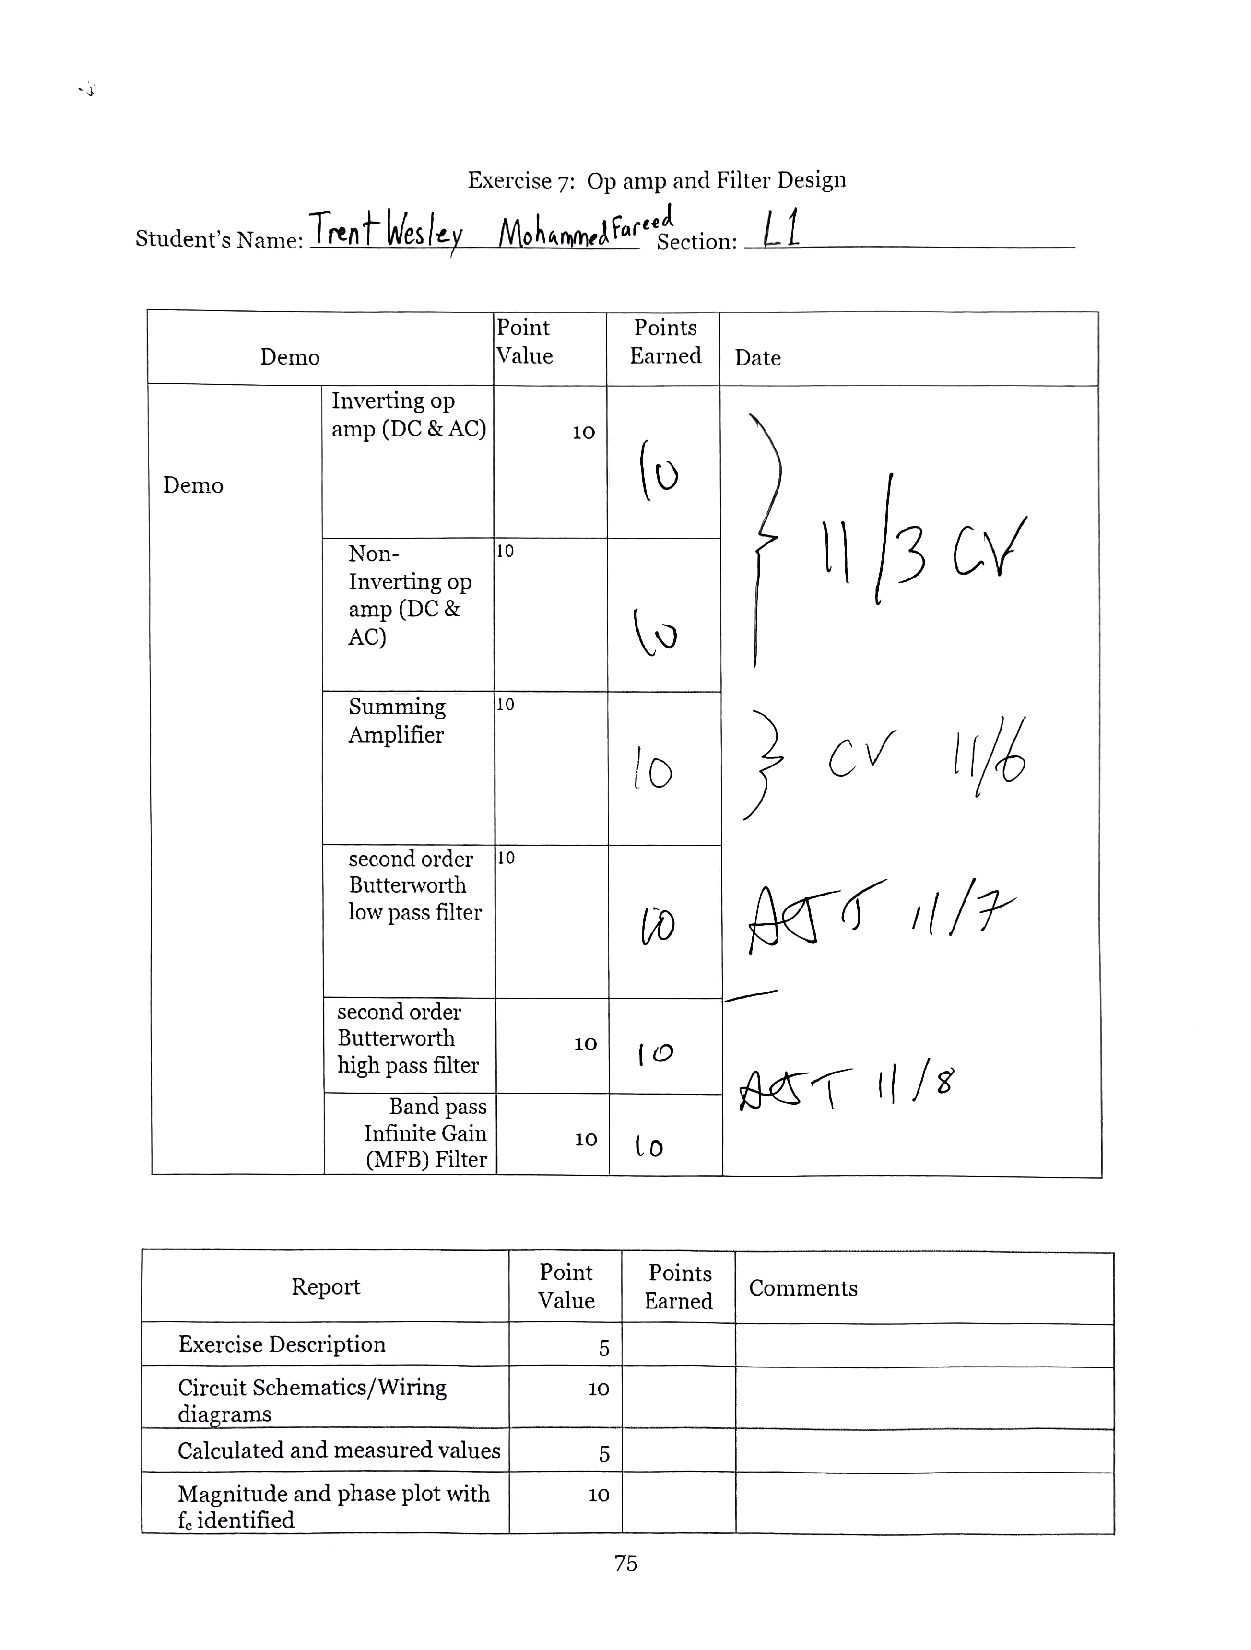
\includegraphics[width=0.75\textwidth]{signoff.pdf}
    \caption{DC Motor Wiring}
    \label{fig:DCMotorWiring}
\end{figure}

\section*{Filters Calculations}

\section*{Filters Plots} % with fc identified

\section*{Questions}

\emph{Question 1.}

Answer.

\bigskip

\emph{Question 2.}

Answer.

\newpage
\begin{figure}[H]
    \centering
    \begin{adjustbox}{center}
        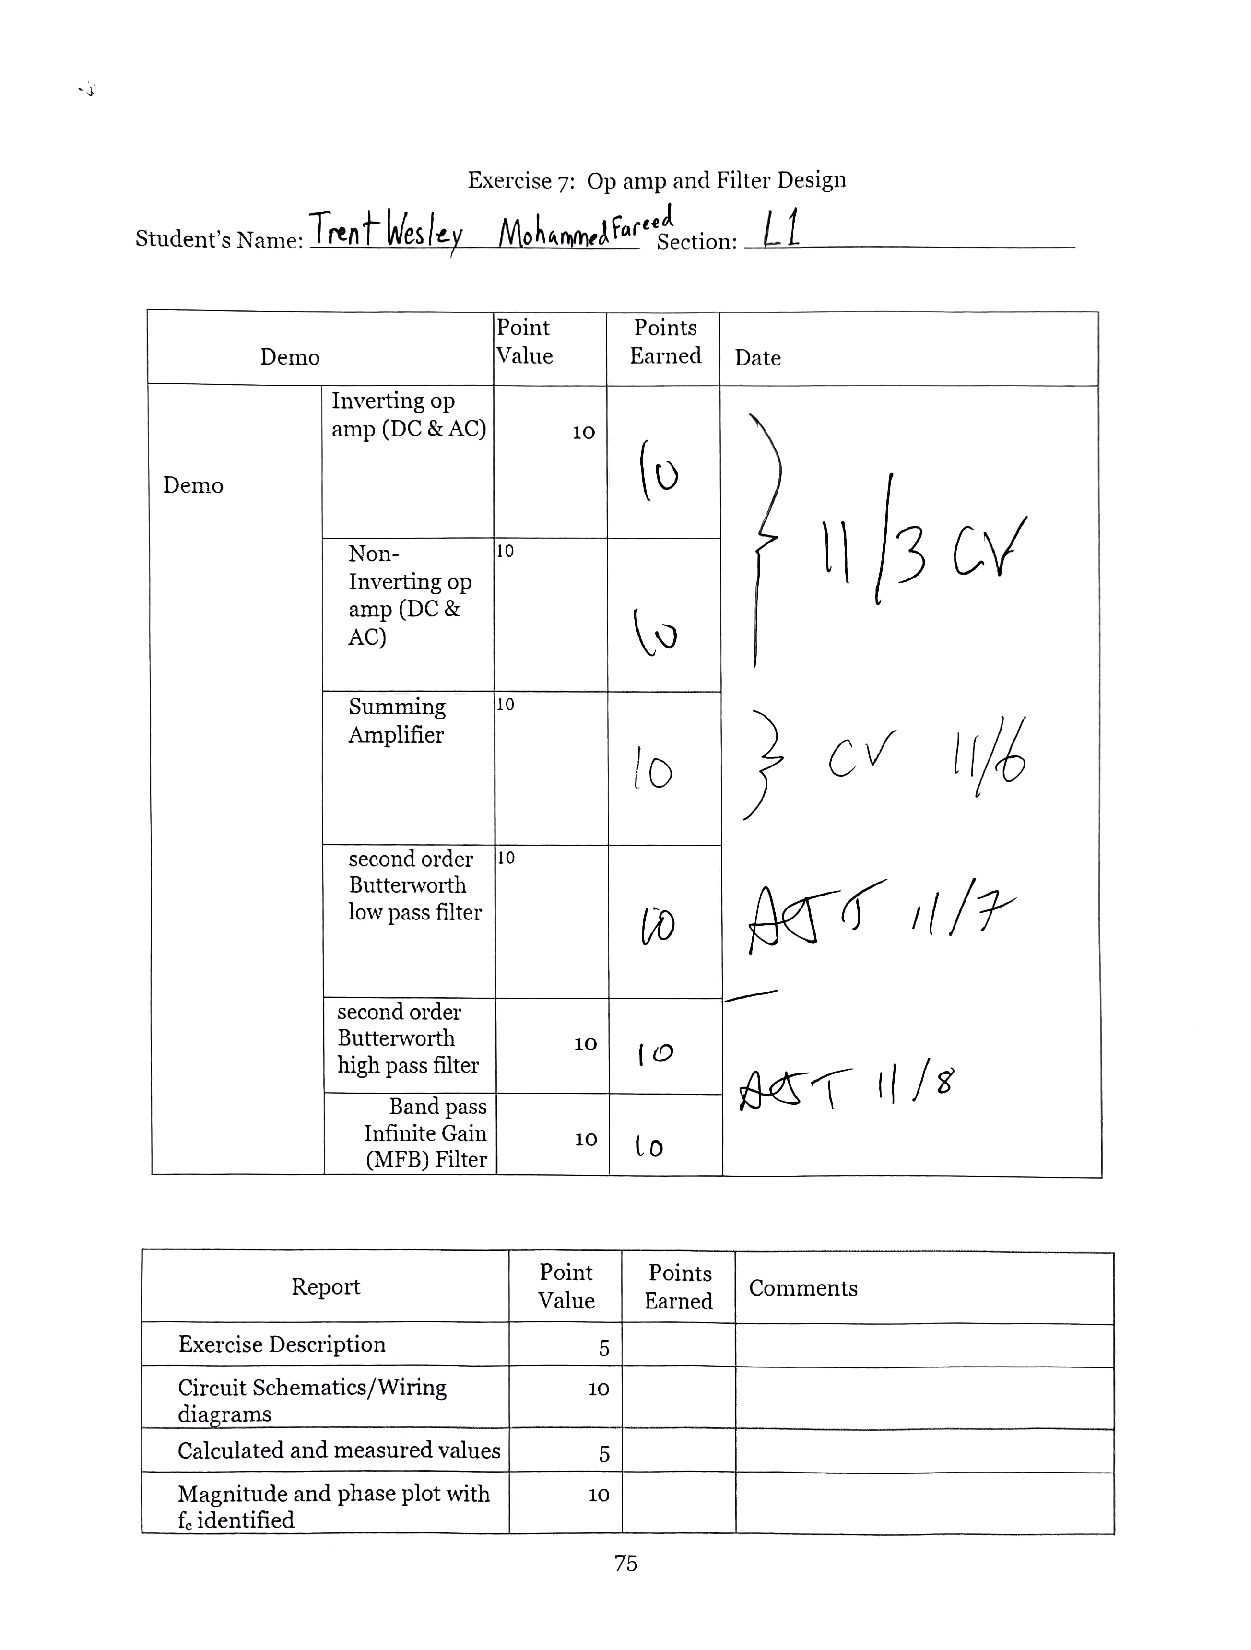
\includegraphics[width=1.26\textwidth]{signoff.pdf}
    \end{adjustbox}
\end{figure}

\end{document}
